\chapter{Descrição do sistema de controle}

O presente trabalho busca controlar a posição de um carro ao longo de uma guia linear. Para realizar essa tarefa, foi escolhida a realimentação de estados como estratégia de controle.

\section{Projeto Realimentação de Estados}

Na realimentação de estados, são determinados requisitos para o sistema, de tal forma que esses correspondem a novos polos do sistema no plano complexo; para tal, uma lei de controle para a mudança dos polos é estabelecida, em que $U(t) = KX(t)$ é o vetor de controle, onde $K \in \mathbb{R}^{n_u \times n}$. A Figura \ref{fig:diagrama_blocos} apresenta o diagrama de blocos com a presença do controlador via realimentação de estados.

\begin{figure}[H]
    \centering
    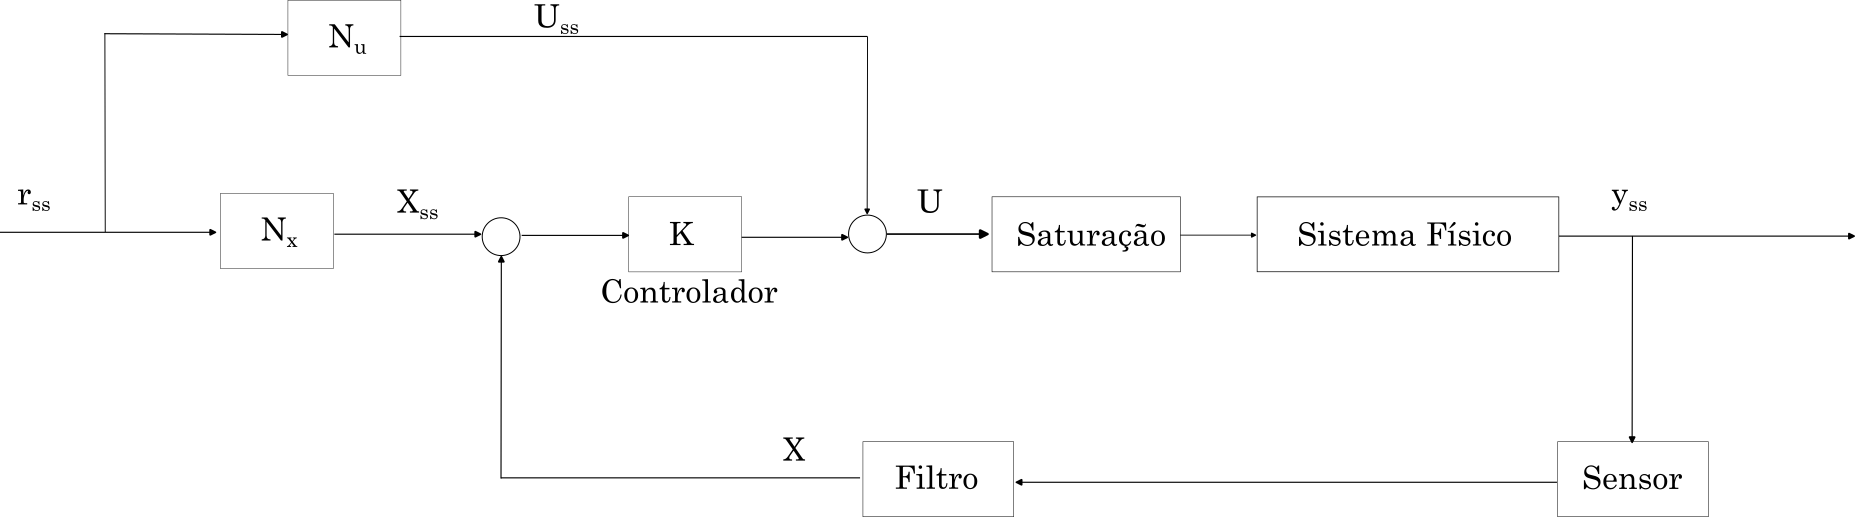
\includegraphics[width=1\linewidth]{figuras/diagrama_blocos.png}
    \caption[Diagrama de blocos da planta]{Diagrama de blocos da planta.}
    \label{fig:diagrama_blocos}
\end{figure}

Conforme mostrado na Figura \ref{fig:diagrama_blocos}, o sistema possui limitações físicas, dessa forma a variável de controle (u) está sujeita a saturação. No caso do sistema estabelecido, a variável de controle é a tensão aplicada no motor CC, medida em Volts, podendo ser na faixa de -12 V a +12 V.

A saída do sensor é submetida ao filtro abordado no Apêndice \ref{apend:1}. A referência ($r_{ss}$) se torna a nova entrada da planta, sendo submetida aos ganhos $N_x$ e $N_u$. A entrada do controlador se torna a diferença entre a referência e a saída atual (y).

\section{Espaço de Estados a tempo discreto}

No capítulo anterior foi elaborado e validado o modelo do espaço de estados a tempo contínuo, unindo as Equações \ref{espaco_estados} e \ref{espaco_estados_saida} com os valores obtidos, obtem-se o seguinte modelo:

\begin{gather}
    \begin{bmatrix}
        \dot{x}_c(t) \\ \ddot{x}_c(t)
    \end{bmatrix}=
    \begin{bmatrix}
        0 && 1 \\ 0 && -5,9313
    \end{bmatrix}
    +
    \begin{bmatrix}
        x_c(t) \\ \dot{x}_c(t)
    \end{bmatrix}
    \begin{bmatrix}
        0 \\ 0,8964
    \end{bmatrix}
    Vm(t)
    \label{espaco_estados1}
\end{gather}

\begin{gather}
    Y(t)=
    \begin{bmatrix}
        1 && 0
    \end{bmatrix}
    \begin{bmatrix}
        x_c(t) \\ \dot{x}_c(t)
    \end{bmatrix}
    \label{espaco_estados_saida1}
\end{gather}

Com o modelo em mãos, se torna necessário discretizar a planta para elaboração e implementação do controlador. A tempo discreto, pode-se representar o sistema do seguinte modo

\begin{equation}
    P :\begin{cases} 
        X(k+1) = \Phi X(k) + \varGamma U(k) \\
        Y(k) = CX(k) + DU(k) \\
        \end{cases}
    \label{modelo_espaco_estados_discreto}
\end{equation}

Durante a identificação dos parâmetros físicos realizada no capítulo anterior, os dados experimentais foram coletados com um período de amostragem de 100 ms. Buscando um bom desempenho do controlador ao mesmo tempo com um custo de implementação baixo, foi decidido que o período de amostragem do modelo discreto seria 10 vezes menor, de forma que

\begin{equation}
    T_s = 10 ms
    \label{periodo_amostragem}
\end{equation}

As Equações \ref{espaco_estados1} e \ref{espaco_estados_saida1} foram discretizadas por meio do comando \textit{c2dm} do software MATLAB, foram usados como argumentos para a função o período de amostragem ($T_s$) e o parâmetro \textit{zoh}, o qual representa o método segurador de ordem zero \cite{franklin2013sistemas}. Assim, a tempo discreto, o sistema é representado por

\begin{gather}
    X(k+1)=
    \begin{bmatrix}
        1 && 0,0097 \\ 0 && 0,9424
    \end{bmatrix}
    X(k)
    +
    \begin{bmatrix}
        0 \\ 0,0087
    \end{bmatrix}
    U(k)
    \label{espaco_estados_d}
\end{gather}

\begin{gather}
    Y(k)=
    \begin{bmatrix}
        1 && 0
    \end{bmatrix}
    X(k)
    \label{espaco_estados_saida_d}
\end{gather}

\section{Requisitos de desempenho}

Em malha fechada, a planta a ser controlada é um sistema de segunda ordem, na literatura de controle, sistemas de segunda ordem apresentam a seguinte resposta à um degrau unitário

\begin{equation}
    Y(s)=\frac{w_n^2}{s(s^2+2\zeta w_n s+w_n^2)}
    \label{resposta_ordem2}
\end{equation}

\noindent sendo $w_n$ a frequência natural e $\zeta$ a taxa de amortecimento do sistema.

Para esse tipo de sistema, o tempo de pico ($t_p$) será

\begin{equation}
    t_p=\frac{\pi}{w_n \sqrt{1-\zeta^2}}
    \label{tempo_pico}
\end{equation}

Já o máximo sobressinal ($M_s$)

\begin{equation}
    M_s=e^\frac{-\zeta \pi}{\sqrt{1-\zeta^2}}
    \label{maximo_sobressinal}
\end{equation}

Foram estipulados como requisitos para o sistema um máximo sobressinal de 83\% ($M_s=0.83$) e 0,32 segundos como tempo de pico ($t_p=0,32$). Com esses valores, as Equações \ref{maximo_sobressinal} e \ref{tempo_pico} formam um sistema de equações com 2 variáveis, isolando $\zeta$ e $w_n$ obtem-se

\begin{equation}
    \zeta = \sqrt{\frac{\ln(M_s)^2}{\pi^2+\ln(M_s)^2}} =  0,0592
    \label{zeta}
\end{equation}

\begin{equation}
    w_n = \frac{\pi}{t_p \sqrt{1-\zeta^2}} = 9,8347
    \label{wn}
\end{equation}